\subsubsection{Árboles de decisión} ~\\

	Desde el punto de vista de las ciencias de la computación y las matemáticas, un árbol es un grafo conexo simple y sin ciclos, y sus propiedades son básicas de la teoría de grafos. Formalmente, sea $G=(V,E)$ un grafo, donde $V$ es un conjunto de vértices o nodos y $E=\{ (v_i, v_j), v_j,v_i \in V \}$ es un conjunto de pares donde cada par representa una arista o rama que conecta a dos nodos. Decimos que un grafo conexo y sin ciclos es un árbol si y sólo si $|E| = |V| - 1$. 
	
%	Además, definimos un \textit{camino} o \textit{path} entre los nodos $v_i, v_j \in V, i \neq j$ en $G$ (lo denotamos $P_{v_i, v_j}^G$), como el conjunto $\{ v_i, v_{i+1}, \dots, v_{j-1}, v_j \}$ de nodos talque  $(v_k, v_{k+1}) \in E, k = i, \dots, (j-1)$. Luego, decimos que $G$ es conexo si $\forall v_i, v_j \in V, i \neq j, \exists P_{v_i, v_j}^G$ y no tiene ciclos si $\forall v_i, v_j \in V, i \neq j, \exists ! P_{v_i, v_j}^G $. 
	
	En un árbol exiten dos tipos de nodos. La diferencía radica en la cantidad de nodos adjacente al mismo o grado del nodo, que denotamos $d(v_i), v_i \in V$. Los nodos con grado $\leq 1$ se denominan hojas y el resto son nodos internos. Los árboles que consideramos en este trabajo tienen un tercer tipo de nodo que llamamos raiz. Los árboles con raiz son muy comunes en el área de aprendizaje automático y formalmente se pueden definir en términos de \textit{generaciones} o \textit{niveles}. Es decir, consideramos al nodo raíz como el nivel 0, los vecinos del mismo constituyen el primer nivel y los que están a distancia $k$, forman el $k$-esimo nivel.
	
	Los árboles, en el área de la computación, son estructuras de datos capaces de almacenar y representar información de forma jerárquica (a través de sus nodos). En general y en especial en el área de aprendizaje supervisado son de mucha utilidad ya que computacionalmente son eficientes a la de buscar información dentro de ellos (a diferencia de otras estructuras de datos). Además, su representación es fácil de interpretar por los hombres y su implementación es sencilla.

	Un árbol de decisión, es una estructura similar a un diagrama de flujo el cual, a través de la evaluación de sus atributos (representados por los nodos del árbol), tiene como objetivo la resolución de un problema. Pueden ser usados para la clasificación (variables discretas) o regresión (variables continuas). En los árboles de decisión, cada nodo representa una característica, cada rama que sale de un nodo representa un valor posible para la característica que representa al mismo y por último las hojas representan la etiqueta de clase (decisión tomada luego de computar todas las características). La clasificación comienza en la raiz, donde se pregunta sobre algun valor de una característica en particular del objeto a analizar. Las diferentes ramas que salen de la  raiz corresponden a las diferentes valores posibles. Basado en la respuesta se continua por la rama hasta el nodo siguiente. La siguiente etapa es realizar una decisión en el nodo en cuestión que puede ser considerado como la raiz del sub-árbol. Se continua de esta manera hasta que se alcanza una hoja, la cual no contiene más preguntas. Cada hoja contiene una etiqueta categórica y al objeto, se le asigna la etiqueta de la hoja que ha alcanzado. Un ejemplo simple se puede observar en la figura \ref{fig: Arbol de decision} donde se representa el problema de si es conveniente ir a jugar al tenis basándose en las características del clima.
		\begin{figure}[htbp]
			\centering
			\fbox{ 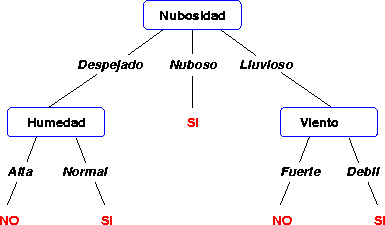
\includegraphics[scale=0.5]{img/tenis_decision_tree.png} }
			\caption{Árbol de decisión.}
			\label{fig: Arbol de decision}
		\end{figure} 
	
	
